\documentclass[a4paper,10pt,twocolumn]{ltjsarticle}
\usepackage[haranoaji]{luatexja-preset}
\usepackage[top=18mm,bottom=20mm,left=17mm,right=17mm,columnsep=8mm]{geometry}
\usepackage{graphicx,booktabs,array,caption,enumitem,xcolor,tikz}
\usetikzlibrary{shapes.geometric}
\setlength{\parindent}{1\zw}
\renewcommand{\baselinestretch}{1.0}
\setlength{\parskip}{0pt}
\renewcommand{\thesection}{\arabic{section}.}
\renewcommand{\thesubsection}{\arabic{section}.\arabic{subsection}.}
\makeatletter
\renewcommand{\section}{\@startsection{section}{1}{\z@}{1.1\Cvs \@plus.4\Cdp \@minus.2\Cdp}{.5\Cvs \@plus.2\Cdp}{\normalfont\gtfamily\bfseries\large}}
\renewcommand{\subsection}{\@startsection{subsection}{2}{\z@}{.8\Cvs \@plus.3\Cdp \@minus.2\Cdp}{.3\Cvs \@plus.1\Cdp}{\normalfont\gtfamily\bfseries\normalsize}}
\makeatother
\captionsetup{font={small,sf},labelsep=space,justification=raggedright,singlelinecheck=false,skip=3pt}
\captionsetup[table]{position=top}
\setlist[itemize]{leftmargin=1.2\zw,itemsep=0pt,topsep=2pt,parsep=0pt}
\setlength{\textfloatsep}{8pt plus 2pt minus 2pt}
\setlength{\floatsep}{8pt plus 2pt minus 2pt}
\setlength{\intextsep}{8pt plus 2pt minus 2pt}
\pagestyle{plain}
\raggedbottom
\begin{document}
\twocolumn[{
\noindent\fbox{\gtfamily\small\ 生成AI論文\ }\par\medskip
\begin{center}
{\gtfamily\bfseries\LARGE 日本の中学校では，考えさせる課題がどれだけ出されているのか：TALIS 2024で54の国・地域と比べる$^{\dagger}$}\par\medskip
{\gtfamily\bfseries\large 批判的思考を要する課題，明確な解のない課題，少人数グループでの共同の解決を求める教員の割合の国・地域間比較}\par\medskip
{\normalsize EduData調査研究グループ$^{*1}$・教育データサイエンス解析班$^{*2}$}\par
{\small オープン教育統計推進プロジェクト$^{*1}$・初等中等STEM教育データ基盤ユニット$^{*2}$}
\end{center}\smallskip
\noindent\begin{minipage}{\textwidth}\small 本研究は，TALIS 2024の公表表から，前期中等教育（日本は中学校）で批判的思考を要する課題，明確な解のない課題，少人数グループでの共同の解決を「頻繁に」または「いつも」求める教員の割合を54の国・地域で比べた．日本は批判的思考を要する課題が24.2\%（27か国のOECD平均61.2\%）で最も低く，明確な解のない課題は28.7\%（同37.1\%）で40番目，少人数グループは53.2\%（同51.2\%）で26番目であった．国・地域の間で，前2者の割合には中程度の正の相関が見られた（\textit{r}=.41，\textit{BF}\textsubscript{10}=12.34）．これらは自己申告の集計値の関連であり，個々の教員の因果を示さない．\par\smallskip
\noindent{\gtfamily キーワード：}TALIS 2024，教員，指導実践，批判的思考，国際比較\end{minipage}\medskip
}]
\let\thefootnote\relax
\footnotetext{\footnotesize 2026年10月執筆\\ $^{\dagger}$How Often Are Lower Secondary Students in Japan Asked to Think? A Comparison with 54 Countries and Economies in TALIS 2024\\ $^{*1}$ Open Education Data Project, Tokyo, Japan\quad $^{*2}$ Educational Data Science Unit, Tokyo, Japan}
\section{はじめに}
\subsection{研究の背景}
生徒に考えさせる指導は，各国の教育改革で論じられてきた．Vieluf et al. (2012)はTALISのデータから指導実践と教育上の革新を検討し，Fullan (2016)は教育の変化の意味を論じた．日本では佐藤 (2012)が学びの共同体による学校改革の構想と実践を示した．Vangrieken et al. (2015)は教員の協働を体系的に整理し，Ertmer and Ottenbreit-Leftwich (2010)は技術活用をめぐる教員の変化に知識，自信，信念，文化が交わることを論じた．Rogers (2003)のイノベーションの普及の枠組みも，新しい実践が広がる過程を考える手がかりとなる．

TALISはOECDが教員と校長を対象に行う国際調査である．2018年の調査の結果は，OECD (2020)と国立教育政策研究所 (2019)が報告している．2024年の結果はOECD (2025)が公表し，前期中等教育の教員の指導実践の割合を国・地域ごとに示した．ただし自己申告の調査であり，言葉の受け取り方や文化の違いが回答に影響しうるため，国際比較は慎重に解釈する必要があるとOECDは注意している．本研究は，考えさせる課題に関わる3つの実践について，日本の位置を整理する．
\subsection{リサーチクエスチョン}
本研究の目的は，TALIS 2024の公表値から，考えさせる課題に関わる指導実践の国・地域による違いと日本の位置を記述することである．
\begin{itemize}
\item RQ1：批判的思考を要する課題・明確な解のない課題・少人数での共同の解決を求める教員の割合は，国・地域でどう違い，日本はどこに位置するか．
\item RQ2：批判的思考を要する課題を出す教員の割合は，明確な解のない課題を出す教員の割合と関連しているか．
\end{itemize}
\section{調査対象および分析方法}
OECDが公表したTALIS 2024の統計表から，前期中等教育（日本は中学校）の教員のうち各実践を「頻繁に」または「いつも」行うと答えた割合（\%）を，54の国・地域について取り込んだ（ベルギーは言語圏別）．オランダ，ニュージーランド，ノルウェー，アルバータ州（カナダ）は，無回答による偏りの危険が高いとOECDが注意している．OECD平均は27か国の平均で，54の国・地域の単純平均とは区別する．

分析単位は国・地域で，各国・地域を同じ重みで扱った．相関はピアソンの \textit{r} と95\%信頼区間，スピアマンの \textit{ρ}，\textit{p}，JZSベイズファクター\textit{BF}\textsubscript{10}で示し，\textit{BF}\textsubscript{10}が3を超えれば関連を支持，1/3未満なら関連がないことを支持とみなした．7指標の全21組を探索的に算出し，研究課題に関わる組を報告する（ボンフェローニの基準は.05÷21，約.0024）．RQ2は，上記4つの国・地域を除いた場合，日本を除いた場合，1か国ずつ除いた場合も計算した．
\begin{table*}[!t]
\caption{主要指標の基本記述統計量}
\centering\small
\begin{tabular}{>{\raggedright\arraybackslash}p{9.2cm}rrrrrr}
\toprule
指標 & \textit{K} & 平均 & \textit{SD} & 中央値 & 最小 & 最大 \\
\midrule
批判的思考を要する課題を出す教員の割合 & 54 & 66.3 & 14.7 & 69.2 & 24.2 & 92.1 \\
明確な解のない課題を出す教員の割合 & 54 & 40.5 & 15.9 & 36.0 & 12.5 & 79.8 \\
少人数グループで共同の解決を求める教員の割合 & 54 & 55.4 & 14.5 & 51.9 & 30.5 & 88.3 \\
学習の計画・管理にデジタル資源を使わせる教員の割合 & 54 & 34.9 & 13.1 & 34.0 & 12.1 & 68.6 \\
デジタル資源で生徒どうしの協働を支える教員の割合 & 54 & 44.1 & 16.0 & 44.6 & 10.6 & 76.5 \\
デジタル資源で学習を支えられる自信のある教員の割合 & 54 & 73.0 & 11.5 & 74.9 & 40.1 & 92.3 \\
AIを仕事で使った教員の割合 & 54 & 41.9 & 14.7 & 41.0 & 13.5 & 75.0 \\
\bottomrule
\end{tabular}
\par\smallskip{\footnotesize 注）単位は\%，\textit{K}は観測数（国・地域）．}
\end{table*}
\begin{table*}[!t]
\caption{主要指標間のピアソンの相関係数と，ベイズファクター}
\centering\small
\begin{tabular}{>{\raggedright\arraybackslash}p{6.4cm}>{\raggedright\arraybackslash}p{6.4cm}rrr}
\toprule
指標 \textit{X} & 指標 \textit{Y} & \textit{r} & \textit{p} & \textit{BF}\textsubscript{10} \\
\midrule
批判的思考を要する課題を出す教員の割合 & 明確な解のない課題を出す教員の割合 & .41 & = .002 & 12.34 \\
批判的思考を要する課題を出す教員の割合 & 少人数グループで共同の解決を求める教員の割合 & .51 & < .001 & 248.71 \\
批判的思考を要する課題を出す教員の割合 & 学習の計画・管理にデジタル資源を使わせる教員の割合 & .42 & = .002 & 13.61 \\
批判的思考を要する課題を出す教員の割合 & デジタル資源で生徒どうしの協働を支える教員の割合 & .57 & < .001 & >1000 \\
批判的思考を要する課題を出す教員の割合 & デジタル資源で学習を支えられる自信のある教員の割合 & .58 & < .001 & >1000 \\
\bottomrule
\end{tabular}
\par\smallskip{\footnotesize 注）\textit{BF}\textsubscript{10}はJZSベイズファクター（3を超えれば関連を支持，1/3を下回れば関連がないことを支持）．全ペアの探索の一部を載せた．}
\end{table*}
\section{結果}
RQ1について，批判的思考を要する課題を出す教員の割合は24.2\%から92.1\%（54の国・地域の平均66.27\%，中央値69.2\%）にわたった．高いのはアラブ首長国連邦（92.1\%），南アフリカ（86.6\%），バーレーン（86.2\%），低いのは韓国（40.4\%），フランドル語圏のベルギー（38.7\%），フィンランド（38.6\%）であった．日本は24.2\%（OECD平均61.2\%）で54番目であり，次に低いフィンランドとも離れていた．明確な解のない課題は12.5\%から79.8\%（平均40.48\%，中央値35.95\%）で，高いのはベトナム（79.8\%），ポーランド（74.1\%），ポルトガル（73.4\%），低いのはチェコ（12.5\%），リトアニア（16.6\%）であった．日本は28.7\%（OECD平均37.1\%）で40番目であった．少人数グループで共同の解決を求める割合は30.5\%から88.3\%（平均55.36\%，中央値51.9\%）で，高いのはアラブ首長国連邦（88.3\%），コロンビア（82.3\%），ベトナム（82.0\%），低いのはフランス語圏のベルギー（30.5\%），スロベニア（31.9\%）であった．日本は53.2\%（OECD平均51.2\%）で26番目と中位にあった．54の国・地域の平均では批判的思考を要する課題が明確な解のない課題を上回るが，日本はこの順が逆であり，このような国・地域は日本を含め3つであった．

RQ2について，批判的思考を要する課題と明確な解のない課題の割合には中程度の正の相関が見られた（\textit{r}=.41，95\%CI [.16, .61]，\textit{ρ}=.44，\textit{n}=54，\textit{p}=.002，\textit{BF}\textsubscript{10}=12.34）．\textit{BF}\textsubscript{10}は関連を支持する範囲にある．この\textit{p}はボンフェローニの基準（約.0024）をわずかに下回るが，21組は互いに独立でなく，余裕も小さいため，探索的な結果として扱う．4つの国・地域を除くと \textit{r}=.46（\textit{n}=50），日本を除くと \textit{r}=.41（\textit{n}=53），1か国ずつ除いた範囲は .39〜.50 であり，日本の極端な値が関連を生んでいるわけではなかった．

なお，少人数グループの割合は，批判的思考（\textit{r}=.51，95\%CI [.28, .69]，\textit{BF}\textsubscript{10}=248.71）とも明確な解のない課題（\textit{r}=.50，95\%CI [.27, .68]，\textit{BF}\textsubscript{10}=155.93）とも中程度の正の相関を示した．3つの実践は，国・地域の間で同じ向きにそろう傾向がある．
\begin{figure}[t]\centering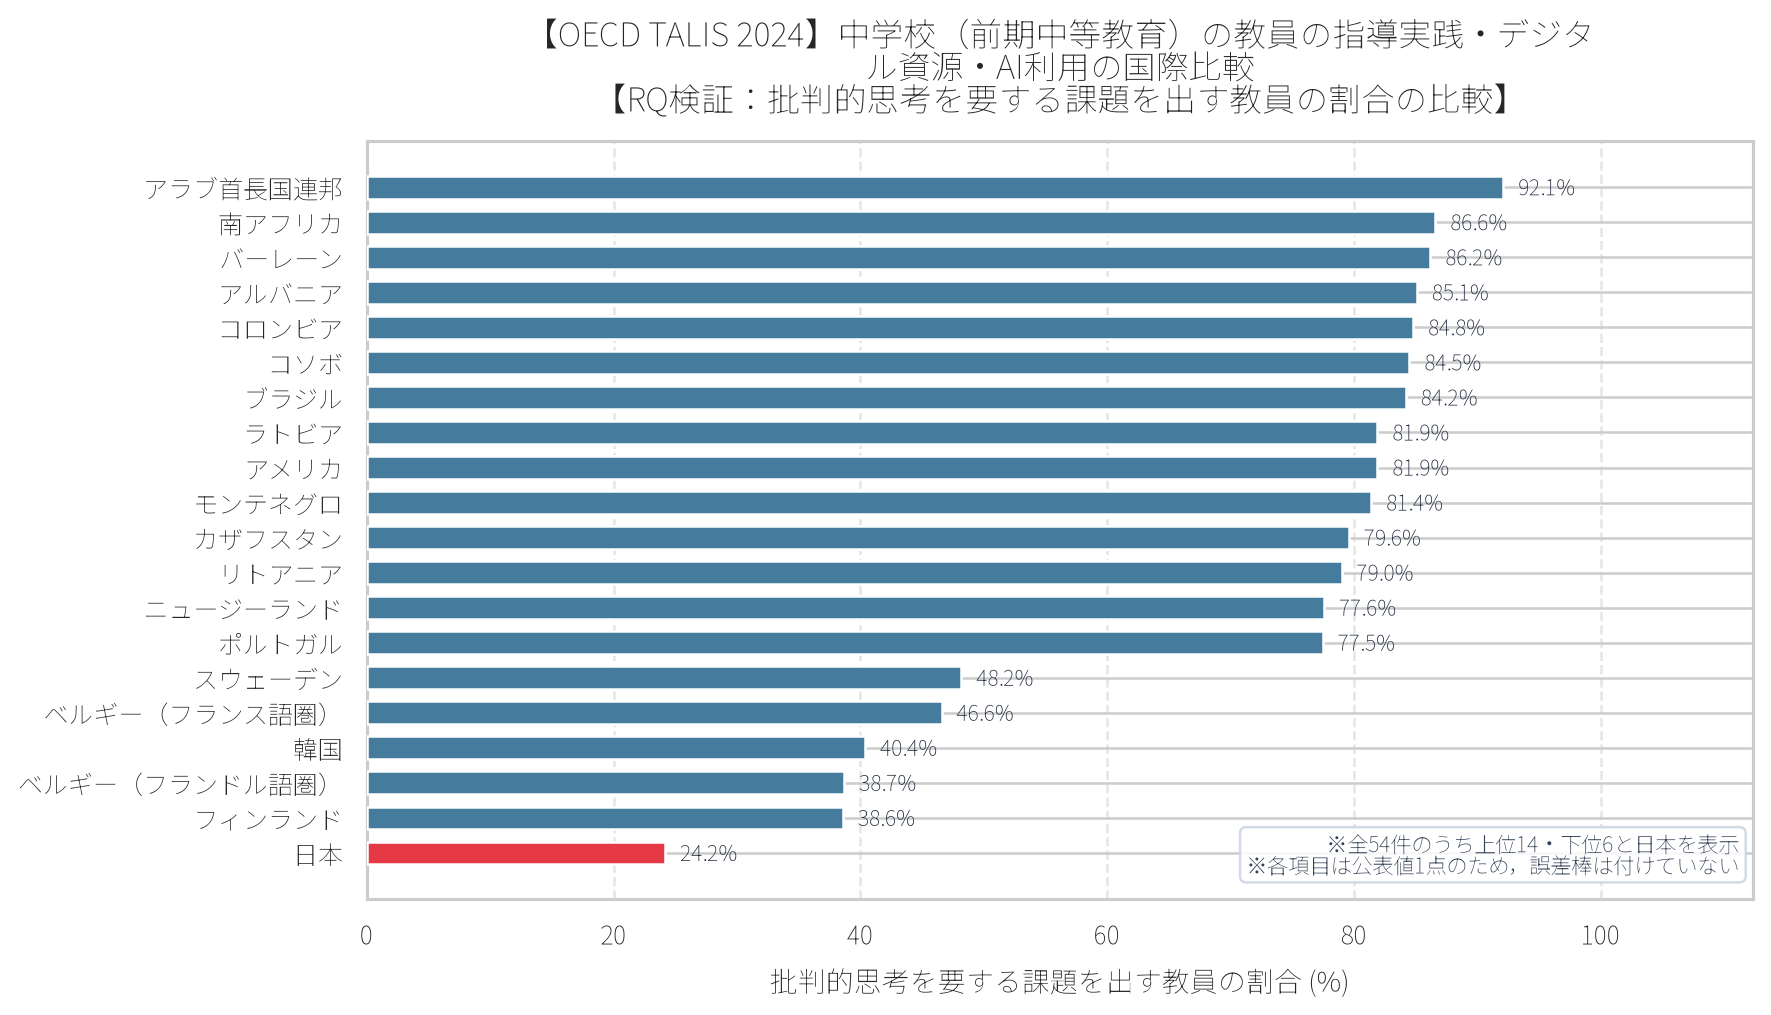
\includegraphics[width=\columnwidth]{chart_oecd_talis_teacher_survey.png}\caption{批判的思考を要する課題を出す教員の割合の値の比較（上位・下位と日本を抜粋）}\end{figure}
\begin{figure}[t]\centering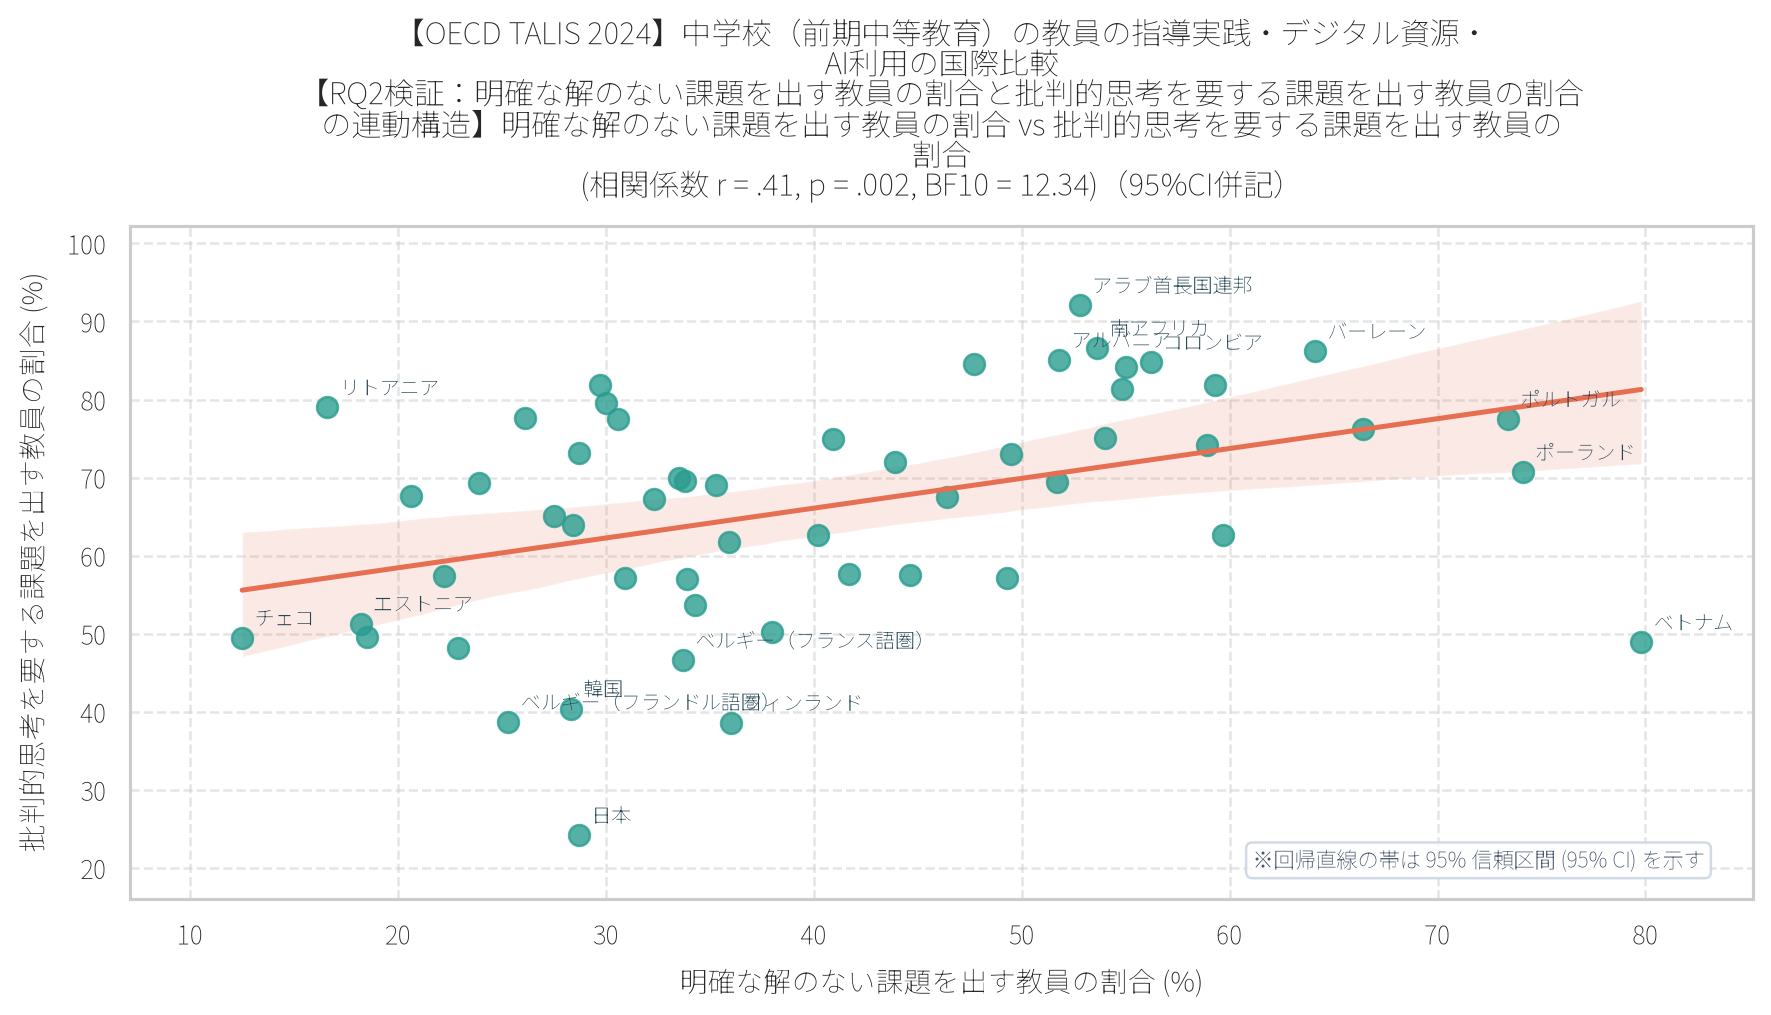
\includegraphics[width=\columnwidth]{chart_secondary_oecd_talis_teacher_survey.png}\caption{明確な解のない課題を出す教員の割合と批判的思考を要する課題を出す教員の割合の関連（回帰直線と95\%信頼区間の帯）}\end{figure}
\section{考察}
RQ1の結果，日本の中学校で批判的思考を要する課題を出すと答えた教員の割合は54の国・地域で最も低く，明確な解のない課題も平均より低かった．一方，少人数グループで共同の解決を求める割合はOECD平均を約2ポイント上回るが，54の国・地域の平均（55.36\%）は下回る中位にあった．これはOECD (2025)の表の範囲で確かめられることである．批判的思考と明確な解のない課題では，27か国のOECD平均と54の国・地域の単純平均のどちらよりも低い．ただし，この低さを授業で考えさせていない証拠とは読めない．日本では「批判的思考」という語の受け取り方が他の国・地域と異なる可能性や，控えめに答える傾向が考えられるが，仮説にとどまり，本研究のデータでは検証できない．低い側に韓国，フィンランド，ベルギーの両言語圏が並ぶことも，単一の説明では捉えにくい．

少人数グループの割合が中位にあることは，佐藤 (2012)の学びの共同体の構想と向きとしては矛盾しないが，両者のつながりはこのデータでは確かめられない．Vangrieken et al. (2015)が整理した教員の協働や，Fullan (2016)が論じた学校の変化も実践の違いに関わりうるが，本研究は扱っていない．

RQ2の正の相関は，批判的思考を要する課題を出す教員の多い国・地域ほど，明確な解のない課題を出す教員も多い傾向を示す．Vieluf et al. (2012)がTALISから指導実践を検討したように，実践どうしの関わりは国際比較の関心事である．しかし本研究の関連は国どうしの違いであり，一方を出す教員ほど他方も出すとは言えない（生態学的誤謬）．3つの実践がそろって高い国・地域と低い国・地域があることから，実践に肯定的に答える傾向の違いが共通して表れている可能性も考えられる．Ertmer and Ottenbreit-Leftwich (2010)は技術活用について教員の変化に信念や文化が交わると論じたが，指導実践の3項目との直接のつながりは本研究では示せない．OECD (2020)と国立教育政策研究所 (2019)は2018年の調査を報告しているが，本研究は同じ質問での変化を確かめていない．

校内で考えさせる課題の例を持ち寄り，「批判的思考」が何を指すかを話し合うことは一つの方向として考えられるが，その効果は確かめられていない．本研究の限界は，(1)集計値のみで個人の因果を特定できないこと，(2)自己申告で言葉や文化の影響を受けうること，(3)4つの国・地域に無回答による偏りの注意があること，(4)経済水準や学校の条件などの交絡を統制していないこと，(5)2024年の1時点であること，(6)全組の探索で多重比較の影響を受けうること，(7)各値の標準誤差を扱わず，順位や約2ポイントの差が誤差の範囲内か分からないこと，(8)ベルギーの2言語圏を別の単位とし，独立でない可能性があること，である．
\section*{参考文献}
\begingroup\scriptsize\setlength{\parindent}{0pt}\raggedright
\par\hangindent=1.5\zw\hangafter=1 ERTMER, P. A. and OTTENBREIT-LEFTWICH, A. T. (2010) Teacher technology change: How knowledge, confidence, beliefs, and culture intersect. Journal of Research on Technology in Education, \textbf{42} (3) ：255-284.\vspace{1pt}
\par\hangindent=1.5\zw\hangafter=1 FULLAN, M. (2016) The New Meaning of Educational Change. Teachers College Press.\vspace{1pt}
\par\hangindent=1.5\zw\hangafter=1 国立教育政策研究所 (2019) 教員環境の国際比較：OECD国際教員指導環境調査（TALIS）2018報告書―学び続ける教員と校長―. ぎょうせい.\vspace{1pt}
\par\hangindent=1.5\zw\hangafter=1 OECD (2020) TALIS 2018 Results (Volume II): Teachers and School Leaders as Valued Professionals. OECD Publishing, Paris. DOI: 10.1787/19cf08df-en\vspace{1pt}
\par\hangindent=1.5\zw\hangafter=1 OECD (2025) Results from TALIS 2024: The State of Teaching. OECD Publishing, Paris. DOI: 10.1787/90df6235-en\vspace{1pt}
\par\hangindent=1.5\zw\hangafter=1 ROGERS, E. M. (2003) Diffusion of innovations (5th ed.). Free Press.\vspace{1pt}
\par\hangindent=1.5\zw\hangafter=1 佐藤学 (2012) 学校を改革する：学びの共同体の構想と実践. 岩波書店.\vspace{1pt}
\par\hangindent=1.5\zw\hangafter=1 VANGRIEKEN, K., DOCHY, F., RAES, E. and KYNDT, E. (2015) Teacher collaboration: A systematic review. Educational Research Review, \textbf{15} ：17-40.\vspace{1pt}
\par\hangindent=1.5\zw\hangafter=1 VIELUF, S., KAPLAN, D., KLIEME, E. and BAYER, S. (2012) Teaching Practices and Pedagogical Innovations: Evidence from TALIS. OECD Publishing, Paris. DOI: 10.1787/9789264123540-en\vspace{1pt}
\endgroup
\section*{Summary}
{\footnotesize\setlength{\parindent}{0pt}Using the published TALIS 2024 tables, we compared, for lower secondary teachers in 54 countries and economies, the share of teachers who frequently or always give tasks that require critical thinking, give tasks with no obvious solution, and ask students to work in small groups on a joint solution. In Japan, 24.2\% of teachers gave tasks requiring critical thinking (OECD average 61.2\%), the lowest of the 54 systems; 28.7\% gave tasks with no obvious solution (OECD average 37.1\%), ranking 40th; and 53.2\% used small-group work (OECD average 51.2\%), ranking 26th. Across countries, the shares for critical-thinking tasks and for tasks with no obvious solution were moderately and positively correlated (r = .41, 95\% CI [.16, .61], BF10 = 12.34), and the association remained when Japan was excluded. Because TALIS is a self-report survey, wording and culture may affect responses. These are associations between country-level aggregates and do not show causation in the behaviour of individual teachers.\par\smallskip KEYWORDS: TALIS 2024, TEACHERS, TEACHING PRACTICES, CRITICAL THINKING, CROSS-COUNTRY\par}
\medskip\noindent\fbox{\parbox{\dimexpr\columnwidth-2\fboxsep-2\fboxrule}{\footnotesize\gtfamily 【付記：生成AIによる自動執筆に関する開示】\\ 本論文は学生への教育目的で作成している．使用しているデータは公的オープンデータである．統計の算出はPythonで行い，文章は生成AI（Anthropic Claude等）を活用して作成した．記載した統計数値は元データに準拠しているが，教育学的な考察や提言の妥当性は，指導現場の実情に応じて，批判的に吟味してほしい．}}
\end{document}
